\chapter{Performance en aplicaciones web}

En el capítulo anterior se definieron los conceptos básicos sobre la performance, las definiciones de métricas, metas y requerimientos de performance, los diferentes tipos
de pruebas y las actividades en las que las pruebas de performance pueden dividirse. En este capítulo nos centraremos en las aplicaciones web y se procederá a
detallar las métricas de performance pertinentes a la hora de analizar qué tan buena es la performance de una aplicación web.


\section{ Métricas de performance. }

En la siguiente sección se definirán las métricas relevantes para las pruebas de performance del proyecto. Estas métricas serán la base para tomar mediciones y compararlas entre 
distintos sitios. Dada la arquitectura típica de una aplicación web, a continuación se presenta una lista de métricas de interés del lado cliente. Estas métricas son producto de
de la investigación del equipo, algunas de ellas están basadas en las herramientas utilizadas posteriormente para realizar las pruebas.

\begin{itemize}
	\item
	\textbf{Tiempo de carga.} Se define como el tiempo desde el pedido inicial hasta la ocurrencia del evento \emph{window load event} o también conocido como \emph{onload}.
	Básicamente se trata del tiempo entre que el usuario realiza un pedido a un sitio y éste carga completamente. Es importante destacar que esta métrica involucra muchos elementos
	de complejidad alta, como AJAX, carga de contenido de terceros y CDNs.
	\item
	\textbf{Tiempo hasta el primer byte recibido.} Se refiere al tiempo transcurrido desde que el navegador utilizado por el usuario realiza un pedido al servidor, hasta que el
	navegador recibe el primer byte de la respuesta del mismo. Vale la pena aclarar que las respuestas con código HTTP de redirección por parte del servidor web no cuentan como
	respuestas al pedido del cliente. Esta métrica sirve como indicador de la capacidad de respuesta de un servidor web u otros recursos de la red.
	\item
	\textbf{Cantidad de pedidos HTTP.} Cantidad de pedidos HTTP necesarios para descargar todos los elementos de un sitio luego del primer pedido realizado. En este punto es
	importante mencionar la regla de oro de la performance del lado cliente ``realizar la menor cantidad de pedidos HTTP posible''. La idea de obtener mediciones sobre esta métrica es
	comparar el comportamiento del sitio en el caso de un usuario que lo visita por primera vez, y luego vuelve a accederlo. En este segundo acceso vale la pena volver a medir
	la cantidad de pedidos para evaluar la efectividad del \emph{caching} del sitio.
	\item
	\textbf{Uso de conexiones persistentes.} Porcentaje de utilización de la directiva \emph{keep-alive} del protocolo HTTP en caso de que sea necesario descargar varios elementos de
	un mismo \emph{host}. Sin la directiva, se estaría cayendo en una penalización fija de tiempo producida por el tiempo de establecimiento de conexión TCP, el cual consta de un
	costo fijo de tiempo por conexión.
	\item
	\textbf{Porcentaje de uso de compresión}. Porcentaje de respuestas del servidor de tipo texto a las cuales se les aplica algún tipo de compresión por parte del servidor. Mientras
	menos pesada sea la respuesta del servidor, más rápido llegará al navegador cliente.
	\item
	\textbf{Uso eficiente de hojas de estilo y javascripts.} Consta en verificar que se utilice solo una hoja de estilos y un archivo de javascripts. Tener un archivo solo para cada tipo de
	recurso ahorra cantidad de pedidos HTTP.
	\item
	\textbf{Cantidad de redirecciones.} Cantidad de redirecciones hasta el pedido final. Según Steve Souders, las redirecciones son muy ineficientes, ya que implican el paso de un RTT
	para cada uno de los pedidos redireccionados, empeorando la experiencia del usuario final.
	\item
	\textbf{Cantidad de \emph{kilobytes} transferidos}. Cantidad de \emph{kilobytes} transferidos por la red, esta métrica puede medirse por pedido HTTP realizado, o evaluando
	por caso de uso de usuario completo.
\end{itemize}


\section{Reglas para mejorar la performance en sitios web}
\label{capitulo3:reglas}

En esta sección se presenta un conjunto de reglas para evaluar la performance de aplicaciones web, que generan un conjunto de buenas prácticas relacionadas con apegarse a las reglas. \cite{souders2007high}.

\subsection{La regla de oro de la performance}

En cualquier esfuerzo por optimizar un sistema, es fundamental realizar un análisis sobre el estado actual de la performance para identificar dónde se pueden llevar a cabo
las mejoras que pueden tener mayor impacto sobre la aplicación.

Al analizar los principales sitios de Estados Unidos, se puede ver la incidencia de la capa de presentación en la performance, su gran potencial para mejoras y la necesidad de centrarse en ella a la hora de optimizar.

\begin{figure}[h!]
\centering
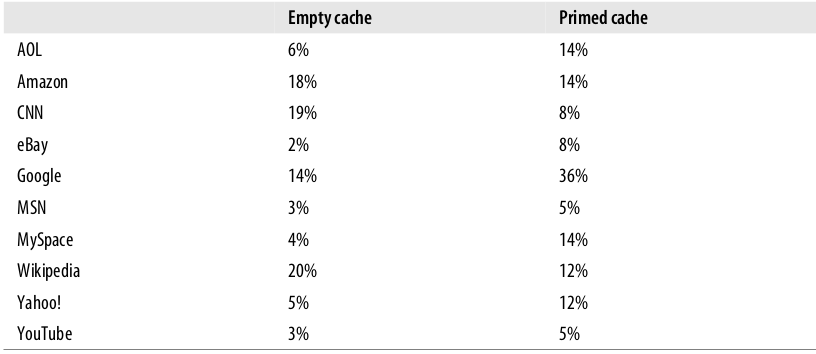
\includegraphics[scale=0.3]{figuras/hpws/tiempos_top10.png}
	\caption{Porcentaje de tiempo utilizado para descargar documento HTML.}
    \label{fig.tiempostopdiez}
\end{figure}

Como se puede apreciar en \ref{fig.tiempostopdiez} solo entre un 10 y un 20\% del tiempo de respuesta es utilizado en descargar el documento HTML, el resto
del tiempo es consumido en la capa de presentación.

Mientras que reduciendo el tiempo de respuesta del \emph{backend} a la mitad, el tiempo de respuesta del usuario se reduciría entre un 5 y un 10\%, si se aumenta la performance de la capa de presentación en un 50\%, el tiempo de respuesta del usuario se reduciría entre un 40 y 45\%.

Adicionalmente, realizar mejoras en la capa de presentación típicamente requiere menos tiempo y recursos. Generalmente mejorar el \emph{backend} involucra rediseñar la arquitectura de la aplicación, optimizar secciones críticas del código, incorporar hardware, distribuir bases de datos, etc. Estos proyectos pueden tardar semanas, incluso meses, en cambio la
mayoría de las mejoras que se pueden implementar para mejorar la performance de la capa de presentación, se pueden realizar en días.

A partir de este análisis realizado sobre el estado de los principales sitios web se define la regla de oro de la performance, que indica que solamente entre un 10 y un 20\% 
del tiempo de respuesta del usuario es utilizado al descargar un documento HTML. El restante porcentaje del tiempo es utilizado en descargar los restantes componentes
en la página.

\subsection{Realizar menos pedidos HTTP}
\label{cap3:reglas:menos_pedidos}

Según la \emph{Regla de oro de la performance} entre el 80 y 90\% del tiempo es utilizado para realizar pedidos HTTP de todos
los componentes referenciados en el documento HTML, desplegar imágenes y ejecutar \emph{scripts}. Por lo tanto reduciendo el número de pedidos HTTP se puede reducir el tiempo
de respuesta.

Cada pedido realizado al servidor implica un \emph{round-trip-time}, que sin importar el ancho de banda entre el usuario y el servidor es una de las penalizaciones más importantes
en la performance de las aplicaciones web, como se puede ver en los resultados obtenidos por Mike Belshe \cite{mike_belshe}. El \emph{round-trip-time} o RTT es el tiempo que
tarda un paquete enviado por un emisor en llegar al receptor más el tiempo que tarda en llegarle un mensaje de confirmación de recepción por parte del receptor.

En base a los datos obtenidos en los experimentos se puede concluir que si un usuario duplica su ancho de banda sin reducir en forma significativa el RTT, la mejora
que percibirá el usuario en la navegación por la web no será muy notoria. Por otro lado, disminuir el RTT sin importar el ancho de banda que se tenga siempre beneficia
la navegación.

A continuación se nombran algunas técnicas para reducir el número de pedidos HTTP sin comprometer el diseño (cantidad de componentes) del sitio.
El empleo de las mismas reduce el tiempo de respuesta para todos los usuarios, pero en particular para aquellos que ingresan por primera vez al sitio y no tienen contenido en la
memoria \emph{cache} del navegador.

\begin{itemize}
\item
Image Maps: Un \emph{image map} permite asociar varias URLs a una sola imagen. La URL de destino es elegida en base a la zona de la imagen donde el usuario realiza un \emph{click}. En lugar de realizar un pedido HTTP por imagen, se realiza uno solo para obtener el \emph{image map}.
\item
CSS Sprites: Esta técnica permite combinar varias imágenes en una sola, de forma más flexible que los \emph{image maps}, ya que no existe la restricción de que las imágenes sean contiguas. Al combinar las imágenes a utilizar en una única imagen se reduce la cantidad de pedidos HTTP, lo que representa una mejora en el tiempo de respuesta.
\item
Inline Images: La técnica \emph{Inline Images} permite incluir imágenes directamente en el sitio sin realizar ningún pedido HTTP adicional al del documento HTML, pero como contrapartida aumenta el tamaño del mismo.
\item
Combinar \emph{Scripts} y hojas de estilo: Una forma de reducir el número de pedidos HTTP consiste en minimizar el número de archivos que se descargan. Combinar todos los \emph{scripts} en un sólo archivo y
todos los CSS en una hoja de estilo reduce de manera considerable el tiempo de respuesta.
\end{itemize}

\subsection{Usar una red de Distribución de Contenido (CDN)}

Una red de distribución de contenido es una colección de servidores web distribuidos en diversos
lugares para entregar de forma más eficiente el contenido a los usuarios.
Los CDNs son utilizados para entregar contenido estático, imágenes, \emph{scripts}, hojas de estilo y contenido \emph{Flash}.

La elección del servidor para hacer entrega del contenido a un usuario específico se basa en la proximidad del usuario a la red. La proximidad de los usuarios al servidor web que contiene la aplicación reduce el tiempo de respuesta de cada pedido HTTP que se realiza al servidor. Si los servidores web que contienen los componentes de la página están próximos al usuario, los tiempos de respuesta de muchos pedidos HTTP pueden ser mejorados.

Por lo tanto, en lugar de rediseñar la aplicación distribuyendo los servidores web que contienen la aplicación, un primer paso más sencillo sería distribuir los servidores
que contienen los componentes de la página, ya que así no solo se obtiene una reducción en los tiempos de respuesta, sino que también el costo y el esfuerzo que esto implica es menor debido a que es muy simple de implementar utilizando redes de distribución de contenido.

\subsection{Agregar el encabezado \emph{Expires}}
\label{cap3:reglas:expires}

Los sitios web contienen una gran cantidad de componentes, por lo que un usuario que visite el sitio por primera vez tendrá que realizar una gran cantidad de pedidos HTTP.
Asignando el encabezado \emph{Expires} especificado en el rfc 2616 \cite{rfc2616} sección 14.21, estos contenidos pueden ser almacenados en la memoria \emph{cache}
de los navegadores, lo que permite ahorrar pedidos HTTP en subsiguientes visitas al sitio.

\begin{figure}[h!]
\centering
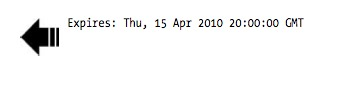
\includegraphics[scale=0.5]{figuras/hpws/expires.jpg}
  \caption{Ejemplo de respuesta HTTP con encabezado \emph{Expires}.}
    \label{fig.expires}
\end{figure}

Los servidores web utilizan el encabezado \emph{Expires} para indicarle al cliente web que puede utilizar la copia actual de un elemento hasta el tiempo especificado por este encabezado, como se puede apreciar en \ref{fig.expires}.
La especificación de HTTP resume este encabezado como \emph{``la fecha o tiempo después del cual es considerado como obsoleto''}.

\subsubsection{\emph{Max-Age} y \emph{mod\_expires}}

Una alternativa para superar las limitaciones que tiene el encabezado \emph{Expires}, es el uso del encabezado \emph{Cache-Control} definido en el rfc 2616 \cite{rfc2616} sección 14.9, el cual
fue introducido en HTTP/1.1. El principal problema con \emph{Expires} es que utiliza
una fecha específica, lo cual requiere una estricta sincronización de relojes entre el servidor y el cliente.

Por otro lado, \emph{Cache-Control} utiliza la directiva \emph{max-age} para especificar cuánto tiempo un componente puede ser almacenado en \emph{cache}.
Define la ventana de validez del componente en la \emph{cache} en segundos. Si desde que el componente fue pedido por primera vez transcurrieron menos de \emph{max-age}
segundos, el navegador utilizará la versión del componente que tiene en su \emph{cache}, evitando de esta forma realizar un nuevo pedido HTTP.
El módulo \emph{mod\_expires} de Apache permite utilizar el encabezado \emph{Expires} de forma similar a \emph{max-age}, expresando la fecha de expiración en términos de
años, meses, semanas, días, minutos o segundos.

\begin{figure}[h!]
\centering
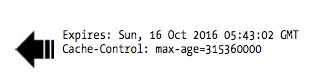
\includegraphics[scale=0.5]{figuras/hpws/cache-control.jpg}
  \caption{Ejemplo de respuesta HTTP con encabezado \emph{Cache-Control}.}
    \label{fig.cache-control}
\end{figure}

Es posible tener ambos encabezados en una respuesta ya que algunos navegadores no soportan HTTP/1.1. Si los dos encabezados están presentes, la especificación
de HTTP dicta que la directiva \emph{max-age} tiene mayor precedencia que el encabezado \emph{Expires}.

Aunque esta práctica debería aplicarse a la mayoría de los componentes de un sitio, actualmente sólo es
común la aplicación del encabezado \emph{Expires} en imágenes. En particular, debería aplicarse el
encabezado a cualquier componente que no tenga cambios frecuentes, incluyendo \emph{scripts}, hojas de estilo y componentes Flash.

\subsubsection{Renombrar archivos}

Cuando se recibe una respuesta con un encabezado \emph{Expires}, el navegador utilizará la versión del componente que contiene en su \emph{cache} hasta
la fecha de expiración. Es por este motivo que el uso de este cabezal reduce enormemente los tiempos de respuesta. En consecuencia, por más que uno actualice un componente
en su servidor, los usuarios que ya visitaron el sitio y tienen el componente en su \emph{cache}, no obtendrán la nueva versión del mismo.

Para asegurar que los usuarios obtengan la última versión de un componente, es necesario cambiar el nombre del archivo del componente. Esta práctica es muy
sencilla si uno genera sus sitios dinámicamente utilizando lenguajes como RoR, Perl, PHP, etc. Es recomendable aplicar esta técnica como parte del proceso de liberación,
agregando el número de liberación a los nombres de los archivos.


\subsection{Comprimir componentes}
\label{cap3:reglas:compresion}

Esta técnica permite reducir los tiempos de respuesta al generar una respuesta HTTP de menor tamaño. De esta forma, el tiempo de transferencia se ve disminuido, ya que se envía
una menor cantidad de paquetes desde el servidor hacia el cliente.

\subsubsection{Funcionamiento}

Desde que surgió HTTP/1.1, los navegadores que soportan compresión indican al servidor los tipos de compresión que soportan mediante la inclusión del encabezado
\emph{Accept-Encoding} en el pedido HTTP. Dicho encabezado se encuentra definido en el rfc 2616 \cite{rfc2616} sección 14.3.

\begin{figure}[h!]
\centering
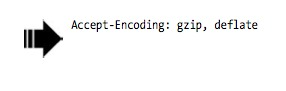
\includegraphics[scale=0.5]{figuras/hpws/accept-encoding.jpg}
  \caption{Ejemplo de un encabezado \emph{Accept-Encoding}.}
    \label{fig.gzip-request}
\end{figure}

Cuando el servidor web recibe un pedido con el encabezado \emph{Accept-Encoding}, puede comprimir la respuesta (en caso de soportarlo) utilizando alguno de los métodos listados
por el cliente en el pedido. El servidor notifica al cliente web que la respuesta esta comprimida agregando el encabezado \emph{Content-Encoding} especificado en el rfc 2616
\cite{rfc2616} sección 14.11 a la respuesta HTTP.

\begin{figure}[h!]
\centering
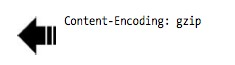
\includegraphics[scale=0.5]{figuras/hpws/content-encoding.jpg}
  \caption{Ejemplo de un encabezado \emph{Content-Encoding}.}
    \label{fig.gzip-respuest}
\end{figure}

La especificación de HTTP/1.1 especifica tres métodos de compresión: \emph{Gzip}, \emph{deflate} y \emph{compress}. Gzip es el más popular y efectivo, es
desarrollado por el \emph{GNU project} y se encuentra estandarizado en el rfc 1952 \cite{rfc1952}. \emph{Deflate} y
\emph{Compress} especificados en el rfc 1950 \cite{rfc1950} son un poco menos efectivos y no son soportados por todos los navegadores.

\subsubsection{¿Qué comprimir?}

Muchos sitios comprimen los documentos HTML, pero es conveniente comprimir también los \emph{scripts} y las hojas de estilo.

La compresión tiene un costo asociado: requiere un uso adicional del CPU del lado del servidor para llevar a cabo la compresión y también del lado del cliente
para descomprimir los archivos que recibe. Para determinar si los beneficios superan a los costos de aplicar ésta técnica, es necesario considerar el tamaño de la respuesta, el
ancho de banda de la conexión y la distancia entre el cliente web y el servidor.

\subsection{\emph{Progressive Rendering}}

Jakib Nielsen deja claro en \cite{Nielsen:1993} la importancia del uso de indicadores de progreso para ayudar a la percepción del
usuario sobre los tiempos de respuesta de una aplicación.

En el caso de los sitios web, la descarga del documento HTML es el indicador de progreso. Los desarrolladores pretenden que el sitio se cargue de forma progresiva, es decir, que el
navegador despliegue contenido lo antes posible, mejorando de esta forma la experiencia de usuario. La ubicación de las hojas de estilo en el documento HTML no afecta
los tiempos de descarga, pero sí los tiempos en que el navegador despliega los elementos en la página.

Los indicadores de progreso brindan información al usuario sobre los tiempos de respuesta de la aplicación. El uso de los mismos ofrece al menos tres ventajas. La primera
ventaja es asegurar que el usuario note que el sistema está en funcionamiento. También indican aproximadamente cuánto tiempo el usuario debe esperar y por último, indican
que la espera sea menos aburrida proporcionando algo para ver.

\subsection{Ubicar las hojas de estilo al comienzo}

El problema de posicionar las hojas de estilo al final del documento HTML es que prohíbe que los navegadores desplieguen progresivamente los componentes del sitio.
En este caso, los navegadores no despliegan elementos para evitar tener que volverlos a desplegar si su estilo cambia debido a una regla de estilo que está definida al final del documento.

En Internet Explorer, colocar las hojas de estilo al final del documento causa el efecto ``Blank White Screen''. Cuando esto ocurre, la página permanece completamente
en blanco hasta que en un momento todo el contenido es desplegado al unísono. Esto significa una mala experiencia de usuario, ya que no se recibe ningún
indicador de que el pedido está siendo atendido de forma correcta.
Para evitar este efecto, es recomendable ubicar las hojas de estilo al comienzo del documento HTML, en la sección \emph{Head} del mismo, de esta forma, los componentes
de la página se desplegarán a medida que son descargados, ya que las reglas de estilo de los mismos ya se encuentran definidas.

\subsection{Ubicar los \emph{scripts} al final del documento HTML}

Con los \emph{scripts} existe un problema similar al que se tiene con las hojas de estilo, pero la solución es opuesta; es mejor posicionarlos al final del documento HTML.
De esta forma los navegadores no solo pueden desplegar progresivamente los componentes del sitio,
sino que también pueden realizar más descargas en paralelo.
El principal problema generado por la descarga de los \emph{scripts} está dado por la limitación de las descargas en paralelo. El mayor impacto en el tiempo de respuesta de un sitio
web está determinado por el número de componentes que tenga, debido a que el navegador debe realizar un pedido HTTP por cada uno de ellos. Cuando la memoria \emph{cache}
del navegador se encuentra vacía, la obtención de cada componente genera un pedido HTTP. La especificación de HTTP/1.1 (rfc 2616 \cite{rfc2616} sección 8.4)
sugiere que los navegadores pueden realizar hasta dos descargas por nombre de \emph{host} en paralelo.

Sin embargo, las descargas en paralelo se deshabilitan cuando el navegador se encuentra descargando un
\emph{script}, en particular el navegador no iniciará nuevas descargas, ni siquiera desde distintos
\emph{hosts}. Una de las razones de este comportamiento es que el \emph{script} puede utilizar la
función \emph{document.write} para alterar el contenido de la página, por lo que el navegador decide esperar para asegurarse de que la página este presentada correctamente.

Otra de las razones por las cuales las descargas en paralelo son bloqueadas mientras se descarga un \emph{script} es para garantizar que los \emph{scripts} sean
ejecutados en el orden correcto. Si varios \emph{scripts} son descargados en paralelo, no existen garantías de que las respuestas de los pedidos lleguen en el
orden especificado.

Si los \emph{scripts} son ubicados al inicio del documento HTML, todo el contenido debajo de ellos no es renderizado y los componentes del sitio no son descargados hasta que los
\emph{scripts} son cargados. Desplegar los componentes del sitio de forma progresiva es fundamental para la experiencia del
usuario, pero los \emph{scripts} lentos y el bloqueo de las descargas en paralelo generan una demora en la respuesta visual que el usuario recibe.

Es por esto, que para mejorar la experiencia del usuario, el mejor lugar para ubicar los \emph{scripts}
es al final del documento HTML. De esta forma no se bloquea la visualización del contenido del sitio y
los elementos que son desplegables son descargados lo más temprano posible.

En algunos casos no es posible ubicar los \emph{scripts} al final del documento, ya que pueden utilizar
la función \emph{document.write} para insertar parte del contenido de la página o por problemas de
\emph{scope}. Una alternativa es utilizar \emph{deferred scripts}. El atributo \emph{DEFFER} indica que
el \emph{script} no realiza una invocación a \emph{document.write}, y por lo tanto los navegadores pueden continuar desplegando y descargando componentes.


\subsection{Evitar \emph{CSS Expressions}}

Las \emph{CSS Expresions} son una forma de definir propiedades de CSS dinámicamente. Eran soportadas por Internet Explorer cinco, seis y siete, pero fueron deprecadas a
partir de Internet Explorer 8. Permiten asignar propiedades CSS como resultado de evaluaciones de código Javascript.

El problema con las \emph{expressions} es que son evaluadas más frecuentemente de lo que la gente espera. No sólo son evaluadas cuando la página es desplegada o
redimensionada, sino también cuando se avanza en la página e incluso cuando el usuario mueve el cursor sobre la misma.

\subsection{Utilizar Javascript y CSS externos}

La utilización de archivos externos de Javascript y CSS, en lugar de posicionarlos \emph{inline} generalmente produce sitios más rápidos. Esto se debe a que los navegadores
pueden almacenar en \emph{cache} los archivos. En caso de que los documentos HTML tengan contenido dinámico, el Javascript y el CSS \emph{inline} es descargado
cada vez que el documento HTML es pedido. En cambio, si el Javascript y el CSS se encuentran en archivos externos que se encuentran en la \emph{cache} del navegador,
el tamaño del documento HTML disminuye sin incrementar la cantidad de pedidos HTTP. El factor más importante a tener en cuenta, es la frecuencia con la cual los
archivos externos son almacenados en \emph{cache} en relación al número de documentos HTML pedidos.

Este factor aunque es difícil de cuantificar, puede ser medido utilizando las siguientes métricas.

\subsubsection{Visitas de páginas}

A menor cantidad de visitas por usuario, mayor la ventaja de utilizar \emph{inline} Javascript y CSS, ya que entre visitas, cualquier archivo externo almacenado en \emph{cache}
puede haber sido borrado de la misma. Por el contrario, si el usuario típico realiza muchas visitas, es más probable que el navegador tenga los componentes externos en su
\emph{cache}. A medida que aumentan las visitas del usuario por mes o por sesión, aumenta el beneficio de utilizar archivos externos de Javascript y CSS.

\subsubsection{Reutilización de componentes}

El uso de archivos externos permite tener una elevada tasa de reutilización de los mismos si varias páginas de un mismo sitio utilizan el mismo Javascript y CSS externo.
En caso que ninguna página comparta el mismo Javascript o CSS, la tasa de reutilización sería más baja, por lo tanto es necesario un análisis de cada sitio en
particular. Si se logra encontrar un balance que resulte en una alta tasa de reutilización, es conveniente utilizar archivos externos, en caso contrario una mejor alternativa
es tener Javascript y CSS \emph{inline}.

El único caso donde es preferible utilizar Javascript y CSS \emph{inline} es en las páginas principales de los sitios. Esto se debe a que estas páginas
tienen un alto número de visitas, menos elementos en el \emph{cache} del navegador y una tasa de reutilización baja. Otro factor que influye en esta decisión, es la
necesidad de que el tiempo de respuesta de estas páginas sea muy reducido para captar la atención del usuario en su primer contacto con el sitio.

\subsubsection{Descargas \emph{Post-Onload}}

Para las páginas principales que derivan en visitas a otras páginas del sitio, se debe utilizar Javascript y CSS \emph{inline} y precargar los archivos externos correspondientes
para las páginas secundarias. Esto se logra descargando dinámicamente los componentes externos una vez que haya terminado de cargar la página principal mediante
el evento \emph{onload}. Esto hace que el navegador agregue en su \emph{cache} los archivos externos anticipando visitas del usuario a otras páginas para reducir el tiempo
de respuesta de las mismas.

\subsubsection{\emph{Dynamic Inlining}}

Si un servidor pudiera saber si un componente se encuentra en el \emph{cache} del navegador, podría decidir si utilizar archivos externos es una estrategia mejor
a incluir las hojas de estilo y el código Javascript \emph{inline} o viceversa.
Retornando una \emph{cookie} que almacena la sesión con el componente buscado, el servidor puede tomar
una decisión sobre qué estrategia tomar en base a la presencia o no de la
misma. En caso de que no se encuentre la \emph{cookie}, se debe utlizar Javascript y CSS \emph{inline} y
en caso contrario, se utiliza el componente externo que se encuentra en la \emph{cache} del navegador.

\subsection{Reducir las búsquedas DNS}

El \emph{Domain Name System (DNS)} traduce nombres de \emph{hosts} a direcciones IP. El navegador no puede descargar elementos desde un \emph{host}
hasta que se complete la búsqueda. Las búsquedas \emph{DNS} tienen un costo, habitualmente toma entre veinte y ciento veinte milisegundos realizar la búsqueda de la
dirección IP de un \emph{host}. El tiempo que toma resolver la consulta depende de la proximidad que se tenga al servidor DNS, la carga que tenga el mismo y el ancho de banda del que se disponga.

\subsubsection{\emph{DNS Caching} y {time to live}}

Los resultados de las búsquedas de \emph{DNS} pueden ser almacenados en \emph{cache} para mejorar la performance. Una vez que un usuario solicita la dirección IP de un \emph{host}
el resultado de la búsqueda permanece en la memoria \emph{cache} del sistema operativo, por lo que los siguientes pedidos al mismo \emph{host} no requieren de una nueva búsqueda.
Por otro lado los navegadores tienen su propia \emph{cache} separada del sistema operativo en la cual almacenan los resultados de las búsquedas \emph{DNS}.
Mientras el navegador mantenga en su \emph{cache} el registro \emph{DNS} no consulta al sistema operativo por dicho registro y de esta forma se reduce el tiempo de búsqueda.
Si el registro no se encuentra en su \emph{cache}, solicita el mismo al sistema operativo, el cual retorna el registro de su \emph{cache} (en caso de tenerlo almacenado) o
se encarga de realizar la consulta a un servidor remoto.

\subsubsection{Factores que afectan el \emph{cache DNS}}

El servidor es el encargado de determinar cuánto tiempo deben ser almacenados en \emph{cache} los registros \emph{DNS} mediante el valor del encabezado \emph{time to live (TTL)}.
Los navegadores por su parte, limitan el número de registros \emph{DNS} que
mantienen en \emph{cache}, independientemente del tiempo que tengan en el mismo.
Esto se debe a que en caso de que el usuario visite muchos sitios en distintos \emph{hosts} en un período corto, los registros \emph{DNS} que se encuentran en \emph{cache}
por más tiempo son descartados para hacer lugar a los nuevos. El impacto que tiene realizar nuevamente la búsqueda de uno de los valores borrados, no es tan importante
ya que existe la posibilidad de que el sistema operativo mantenga el registro en su \emph{cache}.

Cuando el \emph{cache} del cliente (navegador y sistema operativo) no contiene registros \emph{DNS}, la cantidad de búsquedas \emph{DNS} es igual a la cantidad de nombres de \emph{host}
únicos en la página, esto incluye los nombres de \emph{host} en la \emph{URL} de la página, imágenes, \emph{scripts}, hojas de estilo, etc. Reducir el número de nombres de \emph{host}
únicos, reduce la cantidad de búsquedas \emph{DNS}, reduciendo de esta forma el tiempo de espera del usuario.
Potencialmente esto puede reducir la cantidad de descargas en paralelo que se pueden llevar a cabo, por
lo tanto es necesario encontrar un balance entre la cantidad de nombres de \emph{host} utilizados para
maximizar la cantidad de descargas en paralelo y la cantidad de búsquedas \emph{DNS} que esto tiene
como consecuencia.


\subsection{Minimizar Javascript}

\emph{Minification} es una técnica que consiste en remover caracteres innecesarios (comentarios,
espacios en blanco, saltos de línea) del código para reducir su tamaño y mejorar así el tiempo de carga,
debido a que el tiempo de descarga de los archivos es menor. A medida que el uso y el tamaño de los
\emph{scripts} y hojas de estilo aumenta, también lo hacen las ganancias obtenidas al utilizar la técnica \emph{minification}.

La ofuscación es una alternativa a \emph{minification} que, no sólo remueve comentarios y
espacios en blanco, sino que también altera el código, reduciendo nombres de funciones y variables para que el código sea más compacto.

Mientras que la técnica \emph{Minification} es segura y sencilla, la ofuscación es bastante más compleja. Existen tres principales desventajas al ofuscar el código Javascript:
\begin{itemize}
\item \emph{Bugs}
Como la ofuscación altera el código, existe la posibilidad de introducir errores como resultado del proceso.
\item Mantenimiento
Cualquier símbolo que no debe ser modificado (nombres de funciones pertenecientes a una API) debe ser etiquetado para evitar su alteración.
\item \emph{Debugging}
Debido a que el código ofuscado es muy difícil de leer, resulta complicado depurar el código Javascript en el ambiente de producción.
\end{itemize}

\subsection{Evitar \emph{redirects}}
\label{cap3:reglas:redirects}

Un \emph{redirect} especificado en el rfc 2616 de HTTP\\1.1 \cite{rfc2616} sección 10.3, se utiliza para redirigir usuarios de una URL a otra. Existen diferentes motivos para realizarlo,
entre ellos: redirigir a los usuarios a la nueva versión del sitio, rastrear el flujo de tráfico y crear
URLs que sean fáciles de recordar para el usuario.

Los mensajes HTTP del tipo \emph{redirect} tienen un código de estado en el rango de los 3xx. En la especificación de HTTP 1.1, se incorporaron los códigos 303 \emph{See Other}
y 307 \emph{Temporary Redirect} para clarificar el uso del estado 302 \emph{Found}, pero el uso de éstos últimos es casi inexistente.

\begin{figure}[h!]
\centering
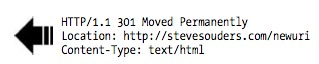
\includegraphics[scale=0.5]{figuras/hpws/redirect.jpg}
	\caption{Ejemplo de una respuesta con código de estado 301.}
    \label{fig.redirect}
\end{figure}

El navegador, al recibir un \emph{redirect} como respuesta dirige automáticamente al usuario a la URL especificada en el encabezado \emph{Location}
especificado en el rfc \cite{rfc2616} sección 14.30. Toda la información necesaria para llevar a cabo el \emph{redirect} se encuentra en los encabezados de la respuesta
y el cuerpo de la misma generalmente está vacío. Si los encabezados \emph{Expires}
o \emph{Cache-Control} están presentes en una respuesta con código 301 o 302, la misma será almacenada en el \emph{cache} del navegador.

Existen además otras formas para redirigir a los usuarios a otra URL. La etiqueta \emph{refresh}
incluida en la sección \emph{head} del documento HTML redirige al usuario después de un número de
segundos especificado en el atributo \emph{content} de la misma.
Javascript también es utilizado para realizar \emph{redirects}, en este caso asignando la URL deseada al atributo \emph{document.location}.

\begin{figure}[h!]
\centering
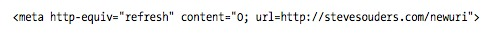
\includegraphics[scale=0.5]{figuras/hpws/meta-refresh.jpg}
	\caption{Ejemplo de una etiqueta refresh.}
    \label{fig.redirect}
\end{figure}

En caso de que sea necesario realizar un \emph{redirect}, la técnica recomendada por \emph{www.w3.org} es utilizar los códigos de estado 3xx de HTTP ya que esto garantiza que el
comportamiento del botón \emph{Atrás} del navegador siga funcionando correctamente.

\subsubsection{Alternativas a los \emph{redirects}}

Uno de los \emph{redirects} más simples de evitar es el que ocurre cuando falta una retrobarra (/) al final de una URL que la requiere. La acción de varios servidores web,
incluyendo Apache, es enviar un \emph{redirect} cuando falta una retrobarra al final de una URL. Una forma de evitar este comportamiento en Apache es utilizar la directiva
\emph{Alias} o el módulo mod\_rewrite.

Otro caso común donde se realizan \emph{redirects} que pueden evitarse es al modificar el \emph{backend}
de un sitio web, ya que las URLs de la nueva implementación pueden variar respecto a las originales. Una
forma de dirigir a los usuarios a la nueva URL es mediante el uso de \emph{redirects}.
A pesar de que la utilización de \emph{redirects} reduce la complejidad para los desarrolladores, como
se mencionó previamente, el uso de esta técnica degrada la experiencia de usuario.

Las siguientes alternativas para integrar dos \emph{backends} agregan más trabajo a los desarrolladores, pero no afectan negativamente la experiencia de usuario.
\begin{itemize}
\item
Uso de \emph{Alias}, mod\_rewrite y \emph{DirectorySlash}.
\item
Si los dos \emph{backends} se encuentran en el mismo servidor, el código mismo puede ser relacionado.
\item
En caso de que el dominio cambie, se puede utilizar un \emph{CNAME} (tipo registro de DNS)  para hacer
que los dos \emph{hosts} referencien a los mismos servidores.
\end{itemize}

\subsection{Eliminar \emph{scripts} duplicados}

Existen dos motivos por los cuales incluir más de una vez el mismo \emph{script} afecta negativamente la performance: se realizan pedidos HTTP innecesarios
y se ejecuta código \emph{Javascript} innecesariamente.

Internet Explorer realiza pedidos HTTP innecesarios cuando se incluye más de una vez un \emph{script} en
un documento HTML y el mismo no está especificado para ser almacenado en \emph{cache}. El navegador realiza un pedido por cada vez que esté incluido el \emph{script} en la página.
En caso de que el \emph{script} este especificado para ser almacenado en \emph{cache}, al recargar la página se realizan dos pedidos HTTP del tipo \emph{Conditional-Get} para
confirmar que la versión del elemento almacenada en el \emph{cache} sigue siendo válida.

La ejecución redundante de código Javascript sucede en todos los navegadores, independientemente de si el \emph{script} está especificado para ser almacenado
en \emph{cache} o no, teniendo como consecuencia el uso innecesario de CPU y memoria.

Una técnica para evitar incluir el mismo \emph{script} más de una vez es implementar un módulo de administración de \emph{scripts}. Este módulo se encarga de incluir
\emph{scripts} y sus dependencias solamente si no fueron incluidos previamente.

\subsection{Configurar \emph{ETags}}

\subsubsection{\emph{Entity Tags (ETags)}}
Las \emph{ETags} especificadas en el rfc \cite{rfc2616} seccion14.19, son un mecanismo utilizado por los servidores y navegadores web para verificar la validez de los componentes
que se mantienen en \emph{cache}. Una \emph{ETag} es un string que identifica una versión específica de un componente, con la restricción de que el \emph{string} debe empezar
y finalizar con comillas.

\begin{figure}[h!]
\centering
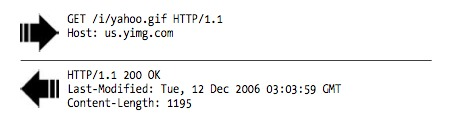
\includegraphics[scale=0.5]{figuras/hpws/etags.jpg}
	\caption{Ejemplo de uso de Etags.}
    \label{fig.redirect}
\end{figure}

El servidor web incluye el encabezado \emph{ETag} en la respuesta con el \emph{string} que identifica la versión del componente solicitado. Cuando el navegador realiza la
validación de la versión del componente que tiene es su \emph{cache}, envía en el pedido el encabezado \emph{If-None-Match} con el \emph{ETag} del componente. En caso de que
los \emph{ETags} coincidan, el servidor responde con un mensaje con código 304 y status \emph{Not Modified}, en caso contrario, responde con un mensaje con código 200
y status \emph{OK} incluyendo la nueva versión del componente. Los \emph{ETags} son útiles en caso de tener que validar componentes en base a una condición diferente
a la última fecha de modificación.

Uno de los principales problemas con las \emph{ETags} es que son específicas para el servidor en el cual fueron creadas. En caso de utilizar un \emph{clúster} de servidores para
balancear la carga de pedidos, si el navegador obtiene el componente de un servidor y después realiza un pedido condicional que es atendido por otro servidor, las
\emph{ETags} no coincidirán y por lo tanto la segunda respuesta tendrá código 200 y contiene al componente.
En caso de tener \emph{n} servidores en un \emph{clúster} con una rotación del estilo \emph{round-robin}, la probabilidad de que una \emph{ETag} de un componente en la memoria
\emph{cache} del usuario coincida con la \emph{ETag} correspondiente al componente en el servidor al cual se realiza el nuevo pedido es \emph{1/n}.

Las \emph{ETags} también degradan la efectividad de los \emph{proxy caches}. La \emph{ETag} de un componente que mantiene un usuario en su \emph{cache} detrás de un
\emph{proxy}, generalmente no coincide con la \emph{Etag} que mantiene en su \emph{cache} el \emph{proxy}, teniendo como consecuencia pedidos innecesarios al servidor
original. Por lo tanto, en lugar de obtener una respuesta con código 304 entre el usuario y el \emph{proxy}, se generan dos respuestas con código 200, una entre el
servidor original y el proxy, y otra entre el \emph{proxy} y el usuario.

Otra de las desventajas de utilizar \emph{ETags} es que el encabezado \emph{If-None-Match} tiene precedencia sobre el encabezado \emph{If-Modified-Since}. En caso de que
se encuentren los dos encabezados en una respuesta, el servidor sólo responde con un mensaje con código 304 si todos los encabezados condicionales son válidos.

\subsection{Almacenar pedidos Ajax en \emph{cache}}

Uno de los principales beneficios de Ajax es que al realizar  los pedidos al servidor web de forma
asincrónica, provee la posibilidad de indicarle al usuario que el sistema está activo sin bloquear la
interfaz de usuario y permitiéndole seguir trabajando.
Sin embargo, en muchas aplicaciones el tiempo de espera del usuario se ve afectado por la forma en que se utiliza Ajax. Un factor clave que influye en el tiempo de espera del usuario, es si
los pedidos Ajax son activos o pasivos.

Los pedidos pasivos se realizan para anticipar una necesidad futura del usuario. Por ejemplo, en un cliente de correo en la web es común realizar un pedido pasivo para
obtener los contactos del usuario, para asegurar que se encuentren en el \emph{cache} para tenerlos disponibles cuando el usuario necesite escribir un correo.
Por otro lado, los pedidos activos se basan en acciones del usuario. Por ejemplo listar los mensajes que cumplen con un criterio de búsqueda.

Los pedidos activos son los que tienen mayor prioridad al optimizar debido a que el usuario debe esperar a que finalicen, pero esto no significa que las optimizaciones a realizar no deban realizarse también para los pedidos pasivos. La principal mejora que se puede realizar es configurar que estos pedidos sean almacenados en \emph{cache} por el navegador, también se pueden
aplicar algunas de las técnicas ya nombradas como comprimir las respuestas, reducir las búsquedas DNS, etc.


\section{Herramientas analizadas.}
\label{capitulo3:herramientas}
Para poder medir y comparar las métricas definidas para la aplicación existen diferentes herramientas que pueden ser utilizadas. A continuación se presentan las herramientas analizadas.

\begin{comment}
\subsection{JMeter}
JMeter es una herramienta de escritorio desarrollada en Java y auspiciada por la Apache Software Foundation. Con este software libre, se pueden definir plantillas para programar baterías de test donde se simulen accesos concurrentes y medir de esta forma los tiempos de respuesta y el rendimiento global del sistema.
Esta herramienta puede ser utilizada como una herramienta de prueba de carga para analizar y medir el desempeño de una variedad de servicios, con énfasis en aplicaciones web.
JMeter puede ser usado como una herramienta de pruebas unitarias para conexiones de bases de datos con JDBC, FTP, LDAP, Servicios web, JMS, HTTP y conexiones TCP genéricas. 
JMeter puede utilizarse para evaluar la performance de recursos estáticos o dinámicos (archivos, servlets, objetos Java, bases de datos y queries, Servidores FTP, entre muchos otros). Se utiliza para simular una carga pesada sobre un servidor, red u objeto para analizar la performance total bajo diferentes tipos de carga. La herramienta puede utilizarse también para obtener análisis gráficos de la performance de la aplicación evaluada o testear el comportamiento de un servidor, script u objeto bajo grandes cargas concurrentes.
JMeter brinda muchas posibilidades y es por ello que es una de las herramientas más utilizadas en el mercado.
La herramienta permite realizar pruebas de carga y performance de diferentes tipos de servidores(Web, HTTP, HTTPS, SOAP. Database via JDBC, Mail-SMTP, POP3,IMAP). Además, es totalmente portable y está desarrollado en un 100\% en java. Además, brinda un framework para el manejo de múltiples hilos permitiendo una muestra concurrente mediante la ejecución de múltiples hilos y permitiendo una prueba simultanea por funcionalidad al definir diferentes grupos de hilos. Además, existen funciones para permitir el ingreso dinámico de datos a una prueba y la posibilidad de manipular dichos datos.
JMeter realiza muchas de las funcionalidades de un navegador al ejecutar una prueba, pero no todas. En particular, JMeter no ejecuta el Javascript que pueda encontrarse en las páginas HTML y tampoco renderiza dichos archivos HTML como lo haría un navegador.
\end{comment}

\subsection{\emph{New Relic}}
\emph{New Relic} \cite{new_relic} es una herramienta para aplicaciones web que permite analizar la performance desde la experiencia del usuario, los servidores y hasta en el código de la aplicación. 
Es una herramienta muy completa que permite entre otras cosas monitorear la experiencia del usuario en tiempo real, analizando los tiempos de carga por aplicación, red y 
renderizado de la página. Además, analiza los tiempos de carga según el navegador y la ubicación geográfica, analiza métricas de performance por página web, entre otras cosas. 
Tiene un mecanismo de alarmas y notificaciones para detectar a tiempo los problemas de performance de la aplicación y genera reportes de errores y disponibilidad del sitio web.

\subsection{\emph{YSlow} y \emph{Page Speed}}
YSlow \cite{yslow} es una herramienta de \emph{Yahoo!} que analiza las páginas web y sugiere formas de mejorar su rendimiento sobre la base de un conjunto de reglas creadas para mejorar sus prestaciones. Sus características más importantes son:
\begin{itemize}
\item
Sugerencias para mejorar el rendimiento de la página.
\item
Resumen de los componentes de la página.
\item
Muestra información sobre la página.
\end{itemize}
Google \emph{Page Speed} \cite{page_speed} es un conjunto de herramientas creadas para ayudar a optimizar el rendimiento de un sitio web. Es una herramienta muy similar a \emph{YSlow}, tomando las mismas métricas y ayudando a analizar e identificar las mejores prácticas para aumentar el desempeño de un sitio web en base a las mismas reglas creadas para mejorar sus prestaciones. Las herramientas de optimización \emph{Page Speed} ayudan a automatizar este proceso.
Estas herramientas son muy similares entre sí, y ambas se basan en la investigación realizada por Steve Souders, experto en el área que trabajó en \emph{Yahoo!} y creó la herramienta \emph{YSlow} y actualmente se encuentra trabajando en Google en la misma área.


Ambas herramientas realizan un \emph{benchmark} de la página web y analizan los componentes para brindar una lista de elementos que pueden ser mejorados para mejorar el tiempo de carga y la velocidad de renderizado. Al utilizar las mismas reglas para realizar sus análisis, su funcionalidad general es muy similar pero presenta algunas diferencias en cuanto a funcionalidades adicionales, como por ejemplo que
\emph{Page Speed} se centra más en el CSS analizando y sugiriendo el uso de selectores, e \emph{YSlow} permite el uso de diferentes perfiles para separar las necesidades de sitios web con mucho tráfico de las de sitios más pequeños.

\subsection{\emph{WebPageTest}}
\emph{WebPageTest} es un proyecto de código abierto que está siendo desarrollado por Google en sus esfuerzos de hacer que la web sea más rápida. Es una herramienta creada inicialmente por AOL para uso interno y que a partir del año 2008 pasó a ser de código abierto.
En su versión online la infraestructura de pruebas es brindada por varias compañías en todas partes del mundo.
La herramienta es similar a las herramientas \emph{YSlow} y \emph{Page Speed}.

\section{Análisis de los diez sitios más visitados de la actualidad.}
\label{capitulo3:sitios_visitados}
Luego de haber analizado las reglas de Steve Souders en la Sección \ref{capitulo3:reglas} y las herramientas que existen actualmente para medir la performance del lado cliente en la Sección \ref{capitulo3:herramientas}, se decidió analizar el estado actual de
los diez sitios más visitados a nivel mundial según el ranking propuesto
por Alexa \cite{alexa}. Se presenta a continuación la lista de sitios ordenadas en forma decreciente por cantidad de visitas:

\begin{enumerate}
	\item
	\textbf{\emph{Google.}} www.google.com
	\item
	\textbf{\emph{Facebook.}} www.facebook.com
	\item
	\textbf{\emph{Youtube.}} www.youtube.com
	\item
	\textbf{\emph{Yahoo}} www.yahoo.com
	\item
	\textbf{\emph{Baidu.}} www.baidu.com
	\item
	\textbf{\emph{Wikipedia.}} www.wikipedia.org
	\item
	\textbf{\emph{Live.(Microsoft)}} www.live.com
	\item
	\textbf{\emph{QQ.}} www.qq.com
	\item
	\textbf{\emph{Twitter.}} www.twitter.com
	\item
	\textbf{\emph{Amazon.}} www.amazon.com
\end{enumerate}

Dado que las reglas escritas por Souders no son demasiado actuales, parece razonable realizar un nuevo análisis acerca de cómo los sitios más concurridos mundialmente se
comportan respecto a la performance. En las siguientes subsecciones se detallará el estado actual de los sitios viendo entre otras cosas puntos de falla comunes y datos
particularmente relevantes. Las herramientas que se utilizaron para recabar datos de performance son \emph{Page Speed}\cite{page_speed} y \emph{Web Page
Test}\cite{web_page_test}.

\emph{Page Speed} es una herramienta \emph{open source} desarrollada por Google la cual se instala como complemento al navegador (disponible tanto para chrome como firefox).
La misma realiza varias pruebas sobre un sitio web, en las cuales toma métricas sobre características de interés sobre la performance del mismo y brinda sugerencias sobre
cómo mejorarla.

Básicamente verifica si el sitio a prueba sigue con las reglas de performance definidas por Souders y dependiendo del grado de cumplimiento otorga un valor
numérico (como máximo cien) que indica que tan bien se comporta el sitio en términos de performance del lado cliente. Un valor elevado implica que existen pocas modificaciones
que se pueden realizar para mejorar la performance, y si por el contrario, el puntaje es bajo el número de mejoras a realizar y el impacto de las mismas es elevado.

Por otro lado, \emph{Web Page Test} fue desarrollada inicialmente por AOL y luego su código fue liberado en 2008 bajo licencia BSD.
A la hora de evaluar, \emph{Web Page Test} toma mediciones sobre métricas muy similares a \emph{Page Speed}. Una de las principales diferencias entre ambas es que
\emph{Web Page Test} permite configurar desde que navegador y ubicación geográfica se desea probar el sitio, además de proveer entre
los resultados los tiempos de respuesta del sitio y la cantidad de pedidos que debieron realizarse.

En la fecha de publicación del libro \emph{Even faster websites} \cite{souders2009even} los sitios más visitados eran los siguientes.

\begin{enumerate}
	\item
	\textbf{\emph{AOL}} www.aol.com
	\item
	\textbf{\emph{Ebay}} www.ebay.com
	\item
	\textbf{\emph{Facebook}} www.facebook.com
	\item
	\textbf{\emph{Google}} www.google.com
	\item
	\textbf{\emph{Live Search}} www.live.com
	\item
	\textbf{\emph{MSN}} www.msn.com
	\item
	\textbf{\emph{My Space}} www.myspace.com
	\item
	\textbf{\emph{Wikipedia}} www.wikipedia.com
	\item
	\textbf{\emph{Yahoo}} www.yahoo.com
	\item
	\textbf{\emph{Youtube}} www.youtube.com
\end{enumerate}

Al analizar la lista del 2007 se encuentran algunas diferencias. Para empezar de los diez sitios más visitados del 2007, hay seis sitios que permanecen en la lista.
Es interesante marcar la entrada de dos sitios de precedencia China con gran cantidad de visitas. Baidu es el sitio de búsquedas más utilizado en China, y QQ
es el sitio de una de las empresas más grandes del mismo país.

Los sitios que salieron del top diez son, My Space (su base de usuarios ha disminuido mucho en los últimos años a manos de otras redes sociales
como Facebook y Twitter). Ebay también se encontraba dentro de los diez sitios más visitados en 2007 pero no ha podido mantenerse, a diferencia de Amazon que no estaba
dentro de los diez más visitados y ahora se encuentra en la décima posición.

\subsection{Interpretación de los resultados.}

A primera vista parecería ser que los sitios del top diez al día de hoy respetan la gran mayoría de las reglas de performance definidas por Souders. Sin embargo, ningún sitio
de la lista cumple todos los consejos propuestos de forma óptima. Para empezar tenemos cuatro sitios que tienen un puntaje de 99/100 utilizando \emph{page
speed}. Estos son, Google, Facebook, Twitter y Baidu, los cuales en su mayoría no cumplen al pie de la letra todas las reglas. Sin embargo, el beneficio que podrían obtener en caso de hacerlo sería marginal. En el extremo más bajo se encuentra Wikipedia con setenta y dos puntos sobre cien.

\subsubsection{Google}

En el caso de la página de inicio de Google, \emph{page speed} le otorga noventa y nueve puntos sobre cien. La única sugerencia propuesta por la herramienta sobre el sitio es minimizar el javascript descargado, lo cual produciría un ahorro del 1\% sobre el total del peso del sitio. Se podría decir que la sugerencia prácticamente
no produce beneficios.

En la imagen a continuación se exponen los resultados obtenidos para las pruebas realizadas por \emph{web page test}.

\begin{figure}[h]
\centering
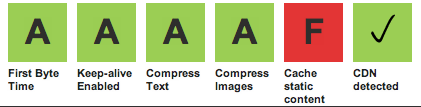
\includegraphics[width=0.5\textwidth]{figuras/lado_cliente/google/page_results.png}
  \caption{Resultados obtenidos por www.google.com.uy}
    \label{fig.google_page_results}
\end{figure}

Este sitio obtiene el peor puntaje en la regla \emph{Cache static content} ya que cuatro de las imágenes que contiene el sitio y el favicon del mismo no contienen los encabezados
\emph{Expires} o \emph{Cache-Control: max-age}, lo cual implica que en cada visita que se haga a la página se enviará un pedido condicional por cada una para verificar si los
elementos no han sido modificados. En particular, el impacto que tiene esta regla en el caso de Google no es de mayor impacto, ya que los elementos que no cumplen con esta regla son pocos
y su tamaño es pequeño.

Por otro lado, cabe destacar que las pruebas realizadas también dependen del navegador dónde se realicen, ya que cuando se accede al sitio de Google con un navegador
distinto a Google Chrome o Mozilla Firefox, la página desplegará un logo del navegador Google Chrome para descargarlo, teniendo que realizarse un pedido HTTP extra.

\subsubsection{Wikipedia}

En la figura \ref{fig.wikipedia_page_results} se pueden apreciar los resultados obtenidos por el sitio \emph{www.wikipedia.org} según la herramienta \emph{web page test}. Este sitio
obtuvo puntaje perfecto en cuatro de las seis reglas \emph{Keep-alive enabled}, \emph{Compress text} y \emph{Compress Images}, \emph{First byte time} y el puntaje
más bajo en la regla \emph{Cache static content}. Por otro lado, este sitio no utiliza una \emph{CDN} (en la imagen esta regla aparece con una \emph{X}), lo cual reduce de
forma considerable su performance.

\begin{figure}[h]
\centering
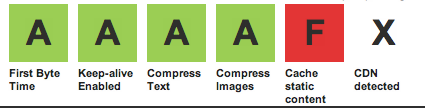
\includegraphics[width=0.5\textwidth]{figuras/lado_cliente/wikipedia/page_results.png}
  \caption{Resultados obtenidos por www.wikipedia.org}
    \label{fig.wikipedia_page_results}
\end{figure}

La herramienta \emph{Page Speed} le brinda un puntaje de setenta y dos sobre cien, y al igual que \emph{web page test} resalta el hecho de que trece de las imágenes (estáticas) que se encuentran en la página y el favicon de la misma no poseen los encabezados \emph{Expires} o \emph{Cache-Control: max-age}, por lo cual en cada visita a
la página se volverá a realizar un pedido para verificar si las imágenes continúan siendo válidas. Si se agregaran estos encabezados se ahorrarían catorce pedidos por visita al sitio, aumentando de forma considerable la performance del mismo.

Otra de las recomendaciones realizadas en este caso por \emph{Page Speed} es que varias de estas
imágenes pueden ser combinadas utilizando la técnica de \emph{CSS-Sprites}, reduciendo de esta forma los
pedidos por imágenes, incluso en la primer visita y con \emph{cache} vacío.

\subsubsection{Facebook}

Facebook obtiene un puntaje perfecto en todas las reglas verificadas por \emph{web page test} a excepción de una, \emph{Compress Images}, en la cual obtiene un 88\%. Esto se
debe a que las dos imágenes que aparecen en la página de inicio como propaganda pueden ser comprimidas para reducir su tamaño y de esta forma aumentar la performance del
sitio. En este caso las ganancias son prácticamente nulas, en el orden de 1.3KB. Los resultados de las distintas reglas según \emph{web page test}
se muestran a continuación.

\begin{figure}[h]
\centering
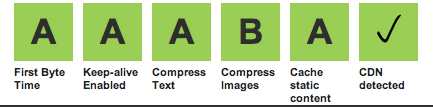
\includegraphics[width=0.5\textwidth]{figuras/lado_cliente/facebook/page_results.png}
  \caption{Resultados obtenidos por www.facebook.com}
    \label{fig.facebook_page_results}
\end{figure}

Otras de las recomendaciones hechas por esta herramienta es que se combinen las cuatro hojas de estilo provistas por facebook en un solo archivo, reduciendo de esta manera
la cantidad de pedidos realizados al sitio.

\emph{Page Speed} le otorga un puntaje de noventa y ocho puntos. Aunque las recomendaciones sean de baja prioridad, ayudan a mejorar la performance del sitio. Por un lado,
además de recomendar la compresión de las imágenes al igual que la herramienta anterior, también recomienda que se especifiquen el largo y ancho de las dos imágenes
que aparecen en la página inicial, para evitar de esta forma tener que calcular estos atributos cuando se esté renderizando la misma.

Por último recomienda utilizar \emph{Defer Parsing} para el siguiente javascript \emph{http://static.ak.fbcdn.net/rsrc.php/v2/y-/r/507fwwUzcWs.js} y para el que se encuentra
de manera \emph{inline} en el cuerpo del documento.

\subsubsection{Youtube}

Al analizar los resultados obtenidos por Youtube según la herramienta \emph{web page test}, se puede apreciar que los mismos no son muy distintos que los del resto de los sitios
previamente analizados. Los mismos se muestran a continuación.

\begin{figure}[h]
\centering
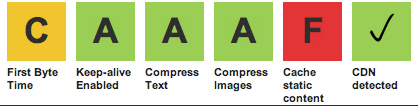
\includegraphics[width=0.5\textwidth]{figuras/lado_cliente/youtube/page_results.png}
  \caption{Resultados obtenidos por www.youtube.com}
    \label{fig.youtube_page_results}
\end{figure}

Uno de los principales problemas encontrados por esta herramienta es el \emph{First time byte}, el cual es aproximadamente trescientos milisegundos mayor al \emph{target time},
lo cual indica la posibilidad de generar mejoras del lado del servidor. Además, el sitio también falla en la regla \emph{Cache static content}, ya que once de los elementos presentes en la página no
contienen los encabezados \emph{Expires} o \emph{Cache-Control:max-age}, lo cual implica que se harán pedidos condicionales para analizar la validez de estos cada vez que se
realice una visita. Por otro lado, el sitio posee diecinueve elementos con un tiempo de expiración de seis horas y siete elementos con veinticuatro horas, esto se debe a que el
contenido del sitio es muy dinámico y cambia constantemente, en particular los videos destacados y recomendados.

Otra de las sugerencias realizadas por la herramienta es combinar las dos hojas de estilo en un solo archivo así como también los archivos con código Javascript, de esta forma
se ahorrarían dos pedidos HTTP en la primer visita el sitio.

Por otro lado, al evaluar el desempeño del sitio con \emph{Page speed} el mismo obtuvo un puntaje de ochenta y nueve sobre cien. Los principales motivos son la falta de fechas de
expiración en algunos componentes de la página, y el trato de las imágenes que realiza el sitio. 
El sitio contiene diez imágenes que son escaladas a un tamaño menor por el navegador y que si fueran provistas por el servidor con el tamaño correcto, permitirían un ahorro de 63.8KB.

Quince de las imágenes que componen el sitio no contienen los atributos \emph{height} y \emph{width} definidos, por lo cual el navegador puede tener que volver a posicionar elementos
del sitio una vez que las imágenes son descargadas.

\subsubsection{Yahoo}

Yahoo a diferencia de la mayoría de los sitios analizados con anterioridad, cumple con la regla \emph{Cache static content} de forma correcta, pero obtiene la peor calificación posible
en el cumplimiento de \emph{Compress Images}. Al igual que Youtube, este sitio no tiene un buen \emph{First time byte}, el mismo es cerca del doble que el \emph{target time},
aproximadamente 513ms. A continuación se muestran los resultados.

\begin{figure}[h]
\centering
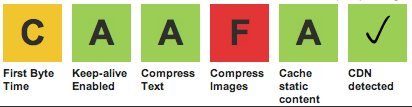
\includegraphics[width=0.5\textwidth]{figuras/lado_cliente/yahoo/page_results.png}
  \caption{Resultados obtenidos por www.yahoo.com}
    \label{fig.yahoo_page_results}
\end{figure}

El principal problema encontrado por esta herramienta son las imágenes que no se encuentran comprimidas. En particular, el sitio cuenta con diecisiete imágenes sin comprimir,
con las cuales se podrían ahorrar 218.4KB. Por otro lado, \emph{Page speed} recomienda englobar las veinticinco imágenes del menú lateral en un \emph{CSS Sprite}, de forma de
ahorrar veinticuatro pedidos la primera vez que se realiza una visita al sitio.
Otra de las recomendaciones hechas por estas herramientas es la combinación de dos archivos de código Javascript en uno solo para ahorrar de esta forma un pedido.

\subsubsection{Baidu}

Este sitio obtuvo uno de los puntajes más altos en relación al resto. \emph{Web page test} detecta dos fallas, la primera es que el favicon de la página no contiene
los encabezados \emph{Expires} o \emph{Cache-Control:max-age}. La segunda sugerencia consiste en el uso de una CDN para proveer los \emph{assets} estáticos. Debajo se encuentran
los resultados obtenidos por este sitio según \emph{Web page test}.

\begin{figure}[h]
\centering
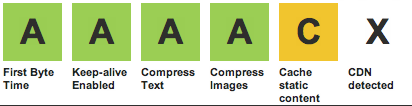
\includegraphics[width=0.5\textwidth]{figuras/lado_cliente/baidu/page_results.png}
  \caption{Resultados obtenidos por www.baidu.com}
    \label{fig.baidu_page_results}
\end{figure}

Por otro lado, \emph{Page speed} brinda sugerencias de baja prioridad. Sugiere utilizar la técnica de \emph{defer parsing}, ya que 40KB del código Javascript es parseado
durante la carga del sitio. Además, sugiere reducir el tamaño del logo principal para ahorrar de esta forma 386B, y especificar el tamaño de las dos imágenes que se
encuentran en el documento para que el navegador no tenga que reposicionar elementos una vez que se descargan estas imágenes.

\subsubsection{Live}

\emph{Web page test} otorga la peor calificación para este sitio al evaluar las reglas \emph{First Time Byte} y \emph{Cache static content}. En la figura \ref{fig.live_page_results}
se puede apreciar el puntaje obtenido por \emph{www.live.com} para todas las reglas.

\begin{figure}[h]
\centering
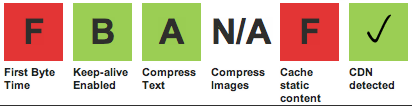
\includegraphics[width=0.5\textwidth]{figuras/lado_cliente/live/page_results.png}
  \caption{Resultados obtenidos por www.live.com}
    \label{fig.live_page_results}
\end{figure}

El motivo por el cual obtiene un puntaje tan bajo en la regla \emph{First Time Byte} es que el mismo tarda 2338ms en llegar, lo que implica que el tiempo de procesamiento
por parte del servidor es muy elevado. Por otro lado, la baja calificación obtenida en \emph{Cache static content} se debe a que una de las hojas de estilo, un archivo javascript
y cuatro imágenes no contienen los encabezados \emph{Expires} o \emph{Cache-Control:max-age}. Además, los javascripts y hojas de estilo correspondientes al login del sitio tienen una expiración de tan solo seis días y veinte horas.

Por otro lado, \emph{Page speed} encuentra varias sugerencias, una de prioridad media y el resto de prioridad baja. La sugerencia de prioridad media consiste en la compresión de
los elementos utilizando \emph{gzip} o \emph{deflate}, ya que una de las hojas de estilo y tres archivos javascript no se encuentran comprimidos, con lo cual se podrían ahorrar
29.6Kb.

Dentro de las sugerencias de menor prioridad, se encuentra la minificación de Javascript, hojas de estilo, el documento HTML y de un archivo .gif cuyo tamaño es mayor que un
paquete, por lo que reduciéndolo se puede reducir la latencia de ese pedido en particular.

Además, sugiere que el \emph{host} \emph{live.com} habilite el encabezado \emph{Keep-alive}, debido a que el mismo provee dos elementos, por lo que se podría
aprovechar la misma conexión para enviarlos y de esta forma ahorrar el \emph{overhead} de tener que establecer una nueva conexión TCP.

\subsubsection{QQ}

El sitio de noticias chino \emph{www.qq.com} no tuvo un buen desempeño en las pruebas realizadas por \emph{Web page test}. En la figura \ref{fig.qq_page_results} se pueden
ver los resultados obtenidos.

\begin{figure}[h]
\centering
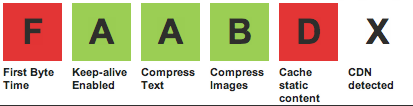
\includegraphics[width=0.5\textwidth]{figuras/lado_cliente/qq/page_results.png}
  \caption{Resultados obtenidos por www.qq.com}
    \label{fig.qq_page_results}
\end{figure}

Uno de los principales problemas de este sitio es el \emph{First time byte} ya que es cinco veces mayor al \emph{Target first byte time}, por lo que existe lugar para realizar
mejoras en el procesamiento del \emph{backend} para que la entrega del primer byte sea más veloz.

Otro de los problemas encontrados, al igual que en varios de los sitios analizados anteriormente, es una baja puntuación en la regla \emph{Cache static content}. Si bien el
sitio cuenta con ocho elementos que no contienen los encabezados \emph{Expires} o \emph{Cache-Control:max-age}, también cuenta con cuarenta y un elementos, de los cuales
cuatro tienen una fecha de expiración menor a cinco minutos, veintitrés elementos con fecha de expiración desde los diez minutos a una hora, doce elementos entre una y dos horas
y por ultimo dos elementos con tres días de expiración, todos plazos de validez demasiado pequeños según la definición de la regla.
Sin embargo, esto se debe a que se trata de un sitio de noticias, donde  las actualizaciones son constantes, por lo cual el puntaje obtenido en esta regla no es tan pertinente, ya que
los plazos cortos de expiración son por este motivo.

Otra de las recomendaciones hechas por esta herramienta es la compresión de las imágenes. Esto se debe a que el sitio cuenta con treinta y ocho imágenes que sin
comprimir o que están parcialmente comprimidas, lo cual permitiría ahorrar 89.9Kb de un total de 483.4Kb de imágenes.

\emph{Page speed} comparte algunas de las recomendaciones hechas por \emph{Web page test}, como la compresión de imágenes y la fecha de expiración de algunos componentes.
Si bien le otorga un puntaje de noventa y dos sobre cien, también sugiere minificar el HTML, el código Javascript y las hojas de estilo, pudiendo ahorrar de esta forma 7.3Kb.
Además, recomienda utilizar técnicas de \emph{Defer Parsing}, debido a que 104.1Kb de código Javascript es parseado durante la carga inicial del sitio y de esta forma se podría reducir el tiempo que tarda el navegador en cargar el sitio.

\subsubsection{Twitter}

Los resultados obtenidos por Twitter para las pruebas de \emph{Web page test} se muestran en la siguiente figura.

\begin{figure}[h]
\centering
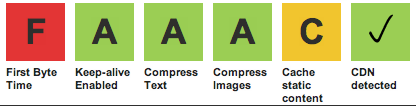
\includegraphics[width=0.5\textwidth]{figuras/lado_cliente/twitter/page_results.png}
  \caption{Resultados obtenidos por www.twitter.com}
    \label{fig.twitter_page_results}
\end{figure}

Se puede ver que el sitio desempeña bien en la mayoría de las reglas a excepción del \emph{First time byte} y \emph{Cache static content}. En el primer caso recibe una calificación \emph{F} a causa de que el valor del \emph{First time byte} es de 912ms cuando el \emph{Target first time byte} es de 414ms.

El sitio obtiene un puntaje medio en \emph{Cache static content} debido a que tres de los componentes tienen una fecha de expiración corta. En particular el
sitio mismo y el siguiente documento \emph{http://api.twitter.com/receiver.html} tienen una fecha de expiración de cinco minutos. Además, el Javascript de google-analytics
que es descargado tiene una fecha de expiración de doce horas.

Otra de las sugerencias realizadas por esta herramienta es la combinación de las dos hojas de estilo utilizadas por el sitio de forma de ahorrar un pedido HTTP. También se sugiere la
compresión de la imagen que es utilizada como fondo, ahorrando de esta forma 10.7Kb.

Por otro lado, \emph{Page speed} le otorga un puntaje de noventa y nueve sobre cien, brindando solo recomendaciones de baja prioridad. Entre ellas se encuentran la minificación
de Javascript y de HTML y la compresión de la imagen de fondo. También recomienda especificar las dimensiones de la misma para facilitar al navegador el proceso de renderizado
de la página.

\subsubsection{Amazon}
El sitio de Amazon obtiene un puntaje perfecto en la mayoría de las reglas verificadas por \emph{Web page test}. La calificación más baja que obtiene es \emph{B} en la regla
\emph{Cache static content}. Todos los resultados se muestran en la siguiente figura.

\begin{figure}[h]
\centering
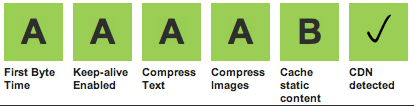
\includegraphics[width=0.5\textwidth]{figuras/lado_cliente/amazon/page_results.png}
  \caption{Resultados obtenidos por www.amazon.com}
    \label{fig.amazon_page_results}
\end{figure}

La razón por la cual obtiene esta calificación en \emph{Cache static content} es debido a que dieciocho componentes de este sitio no tienen los encabezados \emph{Expires}
o \emph{Cache-Control:max-age}. En este conjunto de componentes se encuentran el favicon de la página, un iframe, dos htmls, una imagen de propaganda, seis imágenes del sitio y ocho archivos de javascript. Las imágenes junto con el favicon deberían tener una fecha de expiración muy alta ya que las mismas son estáticas y no cambiarán en el futuro cercano.

Por otro lado, la herramienta recomienda combinar las tres hojas de estilo en una sóla para reducir de esta forma la cantidad de pedidos HTTP que se realizan al cargar la página.

Otra de las recomendaciones realizadas es la compresión de las imágenes ya que ocho de las imágenes contenidas en el sitio se encuentran parcialmente comprimidas o no poseen
compresión alguna, por lo que aplicando esta técnica se pueden ahorrar 44.4Kb, reduciendo el tiempo de descarga. También recomienda utilizar \emph{gzip}, debido a que dos
de los Javascript no se encuentran comprimidos y la mejora que se puede obtener es de 6.1KB.

Las últimas dos recomendaciones son mejorar el \emph{First time byte} que actualmente es de 250ms con un \emph{target first time byte} de 162ms, y utilizar \emph{CDN} para todos los contenidos estáticos, actualmente nueve componentes del sitio no son servidos por \emph{CDN}.

\emph{Page speed} comparte varias de las recomendaciones hechas por \emph{Web page test} y sugiere algunas más. En primer lugar sugiere la utilización de \emph{CSS Sprites}
para seis de las imágenes, incluyendo el logo de Amazon, fotos de iconos de distintas redes sociales y algunas imágenes utilizadas en el menú del sitio.
Por otro lado, sugiere reducir la cantidad de \emph{redirects}. Seis elementos realizan un \emph{redirect} antes de ser obtenidos.

Otra de las recomendaciones obtenidas es la minificación de las hojas de estilo, los Javascripts y el documento HTML, ya que de esta forma se pueden ahorrar aproximadamente 9Kb.
También recomienda especificar las dimensiones de las imágenes. Veinticinco imágenes presentes en el sitio no tienen especificadas sus dimensiones, lo cual puede implicar
que el navegador tenga que calcular el tamaño de algunos componentes y reposicionarlos a medida que renderiza el sitio.

\subsubsection{Otros sitios de alta concurrencia.}

Además de los sitios dentro de los diez más visitados, parece razonable analizar otros sitios de concurrencia alta. El objetivo de este pequeño análisis es mostrar que a pesar de que
algunos sitios sean muy concurridos y que tengan un respaldo económico importante, muchos no siguen las reglas de performance del lado cliente tan bien como podrían.
A modo de ejemplo se mencionan los siguientes sitios.

\begin{itemize}
	\item
	\textbf{\emph{NBA}} www.nba.com
	\item
	\textbf{\emph{The New York Times}} www.nytimes.com
	\item
	\textbf{\emph{CNN}} www.cnn.com
\end{itemize}

\subsubsection{NBA}
El sitio de la NBA marca un puntaje de setenta y dos puntos sobre cien, exactamente el mismo puntaje que el peor sitio de los diez más concurridos. Haciendo una mirada rápida a los
resultados, se puede ver que los errores más graves en cuanto a performance que comete el sitio no son difíciles de solucionar y tienen beneficios potenciales altos.

En primer lugar, el sitio no realiza \emph{caching} de manera correcta sobre las imágenes del menú, lo cual produce que en cada acceso al sitio el navegador deba volver a realizar
pedidos para obtener imágenes estáticas que seguramente no cambien en el corto y mediano plazo. Otro error grave relacionado con las imágenes mencionadas en el punto anterior
es que las mismas no están en un \emph{CSS Sprite} único, lo cual hubiera ahorrado al navegador una cantidad muy grande de pedidos, cumpliendo la regla de oro de la performance del lado cliente.

Una de las fallas más graves del sitio, no detectada en ningún otro sitio durante este análisis es el abuso de redirecciones. En el caso del sitio de la NBA, todos los pedidos de
recursos de avisos publicitarios se encuentran en rutas que terminan en redirecciones, no cumpliendo con una de las reglas de performance definidas por Souders. Otra sugerencia
brindada por la herramienta es habilitar algún tipo de compresión de los componentes, lo cual permitiría al sitio ahorrarse un total de 64\% del tamaño total de transferencia de los
recursos de tipo texto. Otro error bastante grave cometido por el sitio es la cantidad de código javascript que debe cargarse y ejecutarse antes de terminar de cargar la página.
Esto se podría mitigar utilizando algunas de las prácticas de \emph{defer parsing} propuestas por Souders.

\subsubsection{New York Times}

El sitio del diario New York Times marca un puntaje de setenta y ocho puntos sobre cien. Al igual que en el caso de la NBA, el sitio carece de ciertas optimizaciones de performance
que no necesariamente implican un esfuerzo importante para realizarse.

Revisando los resultados rápidamente se puede ver que el sitio tiene varias mejoras de performance pendientes relacionadas con las imágenes que contiene. Por un lado, varias
de las imágenes pueden ser comprimidas para reducir su tamaño. El tamaño de las imágenes de la página principal es más pequeño que el tamaño de las imágenes en el servidor, lo que deriva en que las imágenes que se transfieren sean de un tamaño superior al necesario desperdiciando ancho de banda. Si las
imágenes fueran del tamaño óptimo, el tamaño total de transferencia de las mismas se reduciría en un 53\%, aproximadamente 586.8KB.
Otra mejora posible referente a las imágenes es evitar el re escalado de imágenes por HTML.

Otra mejora sugerida por \emph{Page Speed} es aumentar el tiempo expiración en el cache de las imágenes del sitio. El problema en el caso del New York Times es que la página
principal se actualiza muchas veces al día, y las imágenes cambian en el correr del mismo. Dada la situación, parece innecesario especificar un tiempo de expiración largo para
imágenes que no se mantendrán en el sitio por demasiado tiempo. En cambio, se puede obtener una mejora al combinar las imágenes que pertenecen al menú del sitio en un
\emph{CSS sprite} único para reducir la cantidad de pedidos, este parece ser un error recurrente en la mayoría de los sitios analizados.

Viendo los resultados se pueden encontrar otras mejoras de menos impacto, como por ejemplo obtener recursos de URLs consistentes. Existen cuatro casos de imágenes idénticas
que se obtienen de rutas distintas, lo cual involucra realizar un pedido extra innecesario. Además la carga de javascript inicial es alta y podría reducirse por medio de técnicas de
\emph{Defer parsing} para no bloquear el renderizado del sitio.

Existen otras mejoras de menor impacto, como por ejemplo eliminar una redirección HTTP ahorrándose un pedido.
Otras mejoras posibles serían minificar el código javascript y HTML, aunque el espacio de mejora es bastante reducido.

\subsubsection{CNN}

El sitio de la CNN obtuvo un porcentaje de setenta y ocho puntos sobre cien en la prueba realizada con \emph{Page Speed}. Se pueden ver varias optimizaciones de performance
disponibles en común con los sitios de la NBA y el New York Times.

El problema más grave señalado por las pruebas es nuevamente con el \emph{caching} realizado por el sitio. En el caso de este sitio existen muchos recursos de tipos variados
que tienen un tiempo de expiración fijado en un número muy bajo. En el caso de las hojas de estilo y el código javascript, parecería razonable que se especificaran fechas de
expiración a largo plazo.

Sin embargo, en el caso de las imágenes el problema es un poco más complejo ya que al igual que el sitio del New York Times, las imágenes cambian según las
noticias que se muestren en portada. Las noticias se actualizan de forma regular cada quince minutos, por lo cual no sería razonable aumentar el tiempo de expiración a un valor muy
alto. 

Por otro lado, al igual que con los sitios de la NBA y del New York Times, las imágenes que conforman el menú del sitio son pedidas por el servidor por separado cuando podría
aplicarse la técnica de \emph{CSS sprites} para reducir la cantidad de pedidos.

El sitio de la CNN no tiene habilitada la compresión de elementos de tipo texto. Utilizando alguna técnica de compresión como gzip, se reduciría el tamaño de transferencia
total de estos elementos en un 78\%. El sitio de la CNN tampoco realiza ningún proceso de optimización de imágenes, lo cual podría reducir el tamaño total de transferencia de las
mismas en un 28\%. La cantidad de código javascript descargado cuando se accede a la página principal del sitio es elevado, por lo cual utilizar alguna técnica de \emph{Defer
parsing} podría reducir el tiempo en que el proceso de renderizado se detiene para ejecutar código javascript.

Al igual que en el caso de la NBA, existen cuatro rutas que terminan en redirección, realizando cuatro pedidos más de los necesarios, añadiendo RTTs extra y empeorando la
experiencia del usuario final.

\subsection{Caso de estudio en rails: Diaspora}

Dentro de los sitios más visitados construidos utilizando \emph{Ruby on Rails} se encuentra \emph{Diaspora} (www.joindiaspora.com). Dado que uno de los objetivos del proyecto de grado es identificar buenas
prácticas en aplicaciones de este tipo, se realizó una prueba utilizando \emph{Page Speed} y \emph{Web page test} sobre el sitio. El puntaje otorgado por ambas herramientas se encuentra por debajo del peor puntaje para los diez sitios estudiados anteriormente (Wikipedia).

Los resultados obtenidos por este sitio según \emph{Web page test} son los siguientes:

\begin{figure}[h]
\centering
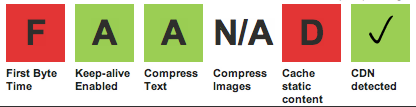
\includegraphics[width=0.5\textwidth]{figuras/lado_cliente/diaspora/page_results.png}
  \caption{Resultados obtenidos por www.joindiaspora.com}
    \label{fig.diaspora_page_results}
\end{figure}

Una de las principales fallas que encuentra \emph{Web test page} es el \emph{First Byte Time}, otorgándole un puntaje de 0 a este sitio. El \emph{target time} (tiempo
necesario para resolver las consultas de DNS, negociaciones de los sockets y SSL más cien milisegundos) para este sitio es de 225ms y el primer byte recibido por el navegador
desde el \emph{backend} tarda 1526ms en llegar. Esto implica que el procesamiento del lado del servidor es bastante lento y puede ser ampliamente mejorado.

El puntaje del sitio según \emph{Page Speed} es de cincuenta y siete sobre cien, a continuación se explican algunas de las causas. El sitio no cumple con ocho de las reglas definidas por la herramienta. Uno de los puntos que produce puntuación más baja es que los contenidos del mismo que están disponibles a través del servicio cloud front de amazon (los
archivos de javascript y CSS) no se comprimen (señalado por \emph{Page Speed} como un problema grave), lo que previene que el sitio reduzca el peso del total de los mismos en un
74\%, aproximadamente 496.6KB. En particular, \emph{Web page test} sugiere además la combinación de estos archivos en dos, uno que contenga el código
javascript y otro las reglas de CSS. En dicha categoría recibe un puntaje de cuarenta y cinco sobre cien.

El segundo punto más importante a mejorar según \emph{Page Speed} es la cantidad de código javascript que el navegador debe procesar. Para ser una página de inicio que solamente
consta de un formulario de ingreso típico del estilo usuario y contraseña, la cantidad de javacript es excesiva. El navegador debe detener el proceso de renderizado para procesar y
ejecutar el código javascript. En este caso parecería razonable utilizar técnicas de \emph{Defer Parsing}, pudiendo retrasar el procesamiento de los javascripts al cargar la página principal,
haciendo sentir al usuario que el sitio está disponible en menos tiempo.

Por otro lado, una de las mejoras más significativas sugerida por \emph{Web page test} es la utilización de los encabezados \emph{Expires} y \emph{Cache-Control:max-age}. En
particular, doce de los componentes de ésta página no contienen estos encabezados, algo considerado como una falla grave, teniendo en lo cuenta que varios de estos componentes son archivos con
código javascript y CSS que no cambia en el corto y mediano plazo, pudiendose ahorrar de esta forma varios pedidos HTTP en próximas visitas a la página.

\emph{Page Speed} también sugiere otras mejoras de menor impacto. Entre ellas se encuentra la omisión de utilizar la bandera \emph{keep-alive} (también sugerida por \emph{Web
page test}) del protocolo HTTP que permite que varios pedidos se realicen en una misma conexión TCP, ahorrando de esta forma el \emph{overhead} que tiene el inicio de una conexión TCP
y el \emph{slow start} de la misma.

Otro punto a mejorar, es la eliminación de código javascript dentro del cuerpo del documento HTML, lo cual produce que el navegador no pueda descargar de forma simultánea o
renderizar otros elementos.



